\clearpage
\subsection{Long-slit spectroscopy, N band}
\label{ssec:recipes_lss_n}
A draft of the reduction cascade is shown in Figs.~\ref{Fig:NLssAssomap1} and \ref{Fig:NLssAssomap2} together with the data processing table (Tables~\ref{Tab:NLssDatProc1} and ~\ref{Tab:NLssDatProc2}). The first part aims to update the static calibration database, in particular the creation of the gain map (\hyperref[Sec:detector_calibration]{\REC{metis_det_lingain}}) and the determination of the \ac{ADC} slitlosses (\hyperref[rec:metis_n_adc_slitloss]{\REC{metis_n_adc_slitloss}}). Both are executed only when an update is required, e.g. after a major instrument interention or on yearly basis. The second part comprises the basic calibrations, e.g. the dark correction and the spectroscopic flatfielding via \ac{RSRF}, followed by the third part, the main calibration steps, incorporating the wavelength calibration (by means of atmospheric lines visible in the respective spectra and the first guess wavelength solution created during \ac{AIT}) and the determination of the response curve for the flux calibration. Therefore the main step of the wavelength calibration is carried out in the recipes \hyperref[rec:metis_n_lss_std]{\REC{metis_N_lss_std}} and \hyperref[rec:metis_lm_lss_sci]{\REC{metis_LM_lss_sci}}. Finally, the telluric absorption correction is applied using the modelling approach with \texttt{molecfit}.
%------------------------------------------------------------------------------------------------------------------
%\subsubsection{Recipes \REC{metis_det_lingain} and \REC{metis_det_dark}}
These recipes aim for detector-specific calibrations and are therefore the same as in the imaging pipeline. Common detector calibrations are described in Section~\ref{Sec:detector_calibration}.
%------------------------------------------------------------------------------------------------------------------
\subsubsection{Recipe \REC{metis_N_adc_slitloss}}
The recipe \hyperref[sssec:adc_slitlosses]{\REC{metis_n_adc_slitloss}} aims to determine the slit losses induced by the fixed \ac{ADC} positions as function of the object position across the slit. The recipe aims to create a table with slitlosses (\hyperref[dataitem:n_adc_slitloss]{\STATCALIB{N_ADC_SLITLOSS}}), which is added to the static database and used in the recipes \hyperref[rec:metis_n_lss_std]{\REC{metis_N_lss_std}}. This recipe is to be carried out only when an update of the database is needed. The algorithm and the workflow of the recipe to determine the slitlosses is given in Section~\ref{sssec:adc_slitlosses}, more information can be found in Section "Calibration of slit losses" in the Calibration Plan \cite{METIS-calibration_plan}. 

%------------------------------------------------------------------------------------------------------------------
\subsubsection{N-LSS Flatfielding recipe \REC{metis_N_lss_rsrf}:}\label{rec:metis_n_lss_rsrf}
The recipe \hyperref[rec:metis_n_lss_rsrf]{\REC{metis_N_lss_rsrf}} aims to create a spectroscopic master flatfield for determining the pixel-to-pixel sensitivity and to enable the order location algorithm (\REC{metis_N_ss_trace}).
\begin{figure}[ht]
  \centering
  
\includegraphics[width=0.5\textheight]{figures/metis_n_lss_rsrf_v0.83.pdf}
  \caption[Recipe: \REC{metis_N_lss_rsrf}]{\REC{metis_N_lss_rsrf} --
    Spectroscopic faltfielding with \ac{RSRF}.}
  \label{Fig:rec_n_lss_rsrf}
\end{figure}

\begin{recipedef}
Name:		& \hyperref[rec:metis_n_lss_rsrf]{\REC{metis_N_lss_rsrf}} \\
Purpose:	& Spectroscopic flatfielding with \ac{RSRF} \\
Type:		& Calibration\\
Requirements: & None \\
Templates:           & \TPL{METIS_spec_n_cal_rsrf} \\
Input data:     & $N\times$ \hyperref[dataitem:n_lss_rsrf_raw]{\RAW{N_LSS_RSRF_RAW}} \\
                & \hyperref[dataitem:persistence_map]{\EXTCALIB{PERSISTENCE_MAP}}  \\
                & \hyperref[dataitem:linearity_geo]{\STATCALIB{LINEARITY_GEO}}  \\
                & \hyperref[dataitem:gain_map_geo]{\PROD{GAIN_MAP_GEO}}  \\
                & \hyperref[dataitem:badpix_map_geo]{\PROD{BADPIX_MAP_GEO}}   \\
                & \hyperref[dataitem:master_dark_geo]{\PROD{MASTER_DARK_GEO}}  \\
Parameters: 	& TBD\\
Algorithm:      & subtract master \ac{WCU} "OFF" frame from illumination frame (done on individual images)\\
                & median/mean filtering of subtracted images\\
                & division by blackbody spectrum\\
                & normalisation to achieve \ac{RSRF}\\
Output data:	&  \hyperref[dataitem:master_n_lss_rsrf]{\PROD{MASTER_N_LSS_RSRF}} (\FITS{PRO.CATG=MASTER_N_LSS_TRSRF}): master flatfield/\ac{RSRF} \\
                & \hyperref[dataitem:median_n_lss_rsrf_img]{\PROD{MEDIAN_N_LSS_RSRF_IMG}}: median map (\ac{QC})\\
                & \hyperref[dataitem:mean_n_lss_rsrf_img]{\PROD{MEAN_N_LSS_RSRF_IMG}}: mean map (\ac{QC})\\

Expected accuracies: & 3\% (cf. \cite{METIS-calibration_plan} and \cite{METIS_calerrbudget})\\
QC1 parameters: & \hyperref[qc:qc_n_lss_rsrf_mean_level]{\QC{QC N LSS RSRF MEAN LEVEL}}: Mean level of the \ac{RSRF}\\
                & \hyperref[qc:qc_n_lss_rsrf_median_level]{\QC{QC N LSS RSRF MEDIAN LEVEL}}: Median level of the \ac{RSRF}\\
                & \hyperref[qc:qc_n_lss_rsrf_intordr_level]{\QC{QC N LSS RSRF INTORDR LEVEL}}: Flux level of the interorder background\\
                & \hyperref[qc:qc_n_lss_rsrf_norm_stdev]{\QC{QC N LSS RSRF NORM STDEV}}: Standard deviation of the normalised \ac{RSRF}\\
                & \hyperref[qc:qc_n_lss_rsrf_norm_snr]{\QC{QC N LSS RSRF NORM SNR}}: \ac{SNR} of the normalised \ac{RSRF}\\
                & more TBD\\
\end{recipedef}

\clearpage
\subsubsection{N-LSS Order detection \REC{metis_N_lss_trace}:}\label{rec:metis_n_lss_trace}
The recipe \hyperref[rec:metis_n_lss_trace]{\REC{metis_N_lss_trace}} aims at detecting the orders and a polynomial fitting of the order locations (see \cite{pis02} and \cite{pis21} for details on the algorithms). The detection and polynomial fitting is based on flatfield frames taken through a pinhole mask, which leads to individual pinhole traces along the entire dispersion direction.

\begin{figure}[ht]
  \centering
  \includegraphics[width=0.5\textheight]{figures/metis_N_lss_trace_v0.83.pdf}
  \caption[Recipe: \REC{metis_N_lss_trace}]{\REC{metis_N_lss_trace} --
    Detection and polynomial fitting of the order location.}
  \label{Fig:rec_N_lss_wave}
\end{figure}

\begin{recipedef}
Name:		& \hyperref[rec:metis_n_lss_trace]{\REC{metis_N_lss_trace}} \\
Purpose:	& Detection of order location \\
Type:		& Calibration\\
Requirements: & None \\
Templates:           & \TPL{METIS_spec_n_cal_InternalWave} \\
Input data:     & $N\times$ \hyperref[dataitem:n_lss_rsrf_pinh_raw]{\RAW{N_LSS_RSRF_PINH_RAW}} \\
                & \hyperref[dataitem:persistence_map]{\EXTCALIB{PERSISTENCE_MAP}}  \\
                & \hyperref[dataitem:linearity_geo]{\STATCALIB{LINEARITY_GEO}}  \\
                & \hyperref[dataitem:gain_map_geo]{\PROD{GAIN_MAP_GEO}}  \\
                & \hyperref[dataitem:badpix_map_geo]{\PROD{BADPIX_MAP_GEO}}   \\
                & \hyperref[dataitem:master_dark_geo]{\PROD{MASTER_DARK_GEO}}  \\
                &  \hyperref[dataitem:master_n_lss_rsrf]{\PROD{MASTER_N_LSS_RSRF}} \\
Parameters: 	& polynomial degree\\
Algorithm:      & Detection of the order edges\\
                & Polynomial fitting\\
Output data:	& \hyperref[dataitem:n_lss_trace]{\PROD{N_LSS_TRACE}} (\FITS{PRO.CATG=N_LSS_TRACE}): Polynomial coefficients\\
Expected accuracies: & (TBD)\\
QC1 parameters: & \hyperref[qc:qc_n_lss_trace_lpolydeg]{\QC{QC N LSS TRACE LPOLYDEG}}: Degree of the polynomial fit of the left order edge\\
                & \hyperref[qc:qc_n_lss_trace_lcoeff<i>]{\QC{QC N LSS TRACE LCOEFF<i>}}: $i$-th coefficient of the polynomial of the left order edge\\
                & \hyperref[qc:qc_n_lss_trace_rpolydeg]{\QC{QC N LSS TRACE RPOLYDEG}}: Degree of the polynomial fit of the right order edge\\
                & \hyperref[qc:qc_n_lss_trace_rcoeff<i>]{\QC{QC N LSS TRACE RCOEFF<i>}}: $i$-th coefficient of the polynomial of the right order edge\\
                & \hyperref[qc:qc_n_lss_trace_intordr_level]{\QC{QC N LSS TRACE INTORDR LEVEL}}: Flux level of the interorder background\\
                & \QC{TBD}: TBD\\
\end{recipedef}

\clearpage

%------------------------------------------------------------------------------------------------------------------
\subsubsection{N-LSS standard star recipe \REC{metis_N_lss_std}:}\label{rec:metis_n_lss_std}
This recipe aims at processing standard stars used for the absolute flux calibration and (optionally) for the telluric feature removal: As first step the detector master calibration files derived previously are applied followed by the background subtraction, if needed the distortion correction (\hyperref[dataitem:n_lss_dist_sol]{\PROD{N_LSS_DIST_SOL}}), and
the wavelength calibration by means of the first guess solution (\hyperref[dataitem:n_lss_wave_guess]{\PROD{N_LSS_WAVE_GUESS}}) and the telluric sky lines (c.f. Sect.\,8.5 in \cite{DRLS}). Then the recipe removes sky background, extracts the standard star spectrum object and collapses the 2D to 1D spectra. In case the \ac{STD} is used only for the flux calibration, a telluric correction is required to better compare the corresponding model spectrum. This is done by means of the standard star observations itself or (optionally) with a synthetic transmission curve (either a standard curve derived by the ESO Skycalc Tool\footnote{\url{https://www.eso.org/observing/etc/bin/gen/form?INS.MODE=swspectr+INS.NAME=SKYCALC}}, a standard curve (\hyperref[dataitem:n_synth_trans]{\STATCALIB{N_SYNTH_TRANS}}) or \texttt{molecfit}. It is on the user's decision whether the standard star is used for the absolute flux calibration only, or also used for the telluric correction of the science target. The response function is then calculated as ratio of the measured 1d-\ac{STD} spectrum and a detailed model containing absolute flux information.

Please note that the procedure of the \ac{STD} handling changes when the classical method for the telluric correction is chosen. The reason is that in the response function, also the telluric features of the \ac{STD} star have to be present to be able to apply a combination of the telluric absorption removal and the conversion towards physical flux units (cf. Section~\ref{ssec:tellcorr}). In the case of using \texttt{molecfit}, a telluric correction is applied to the \ac{STD} spectrum to better determine the response function and only the response is delivered to the science recipes. In case of the classical approach with a \ac{STD}, the response function shall also contain the telluric features of the \ac{STD}, and therefore a telluric correction beforehand is counterproductive.\\

\begin{figure}[ht]
  \centering
  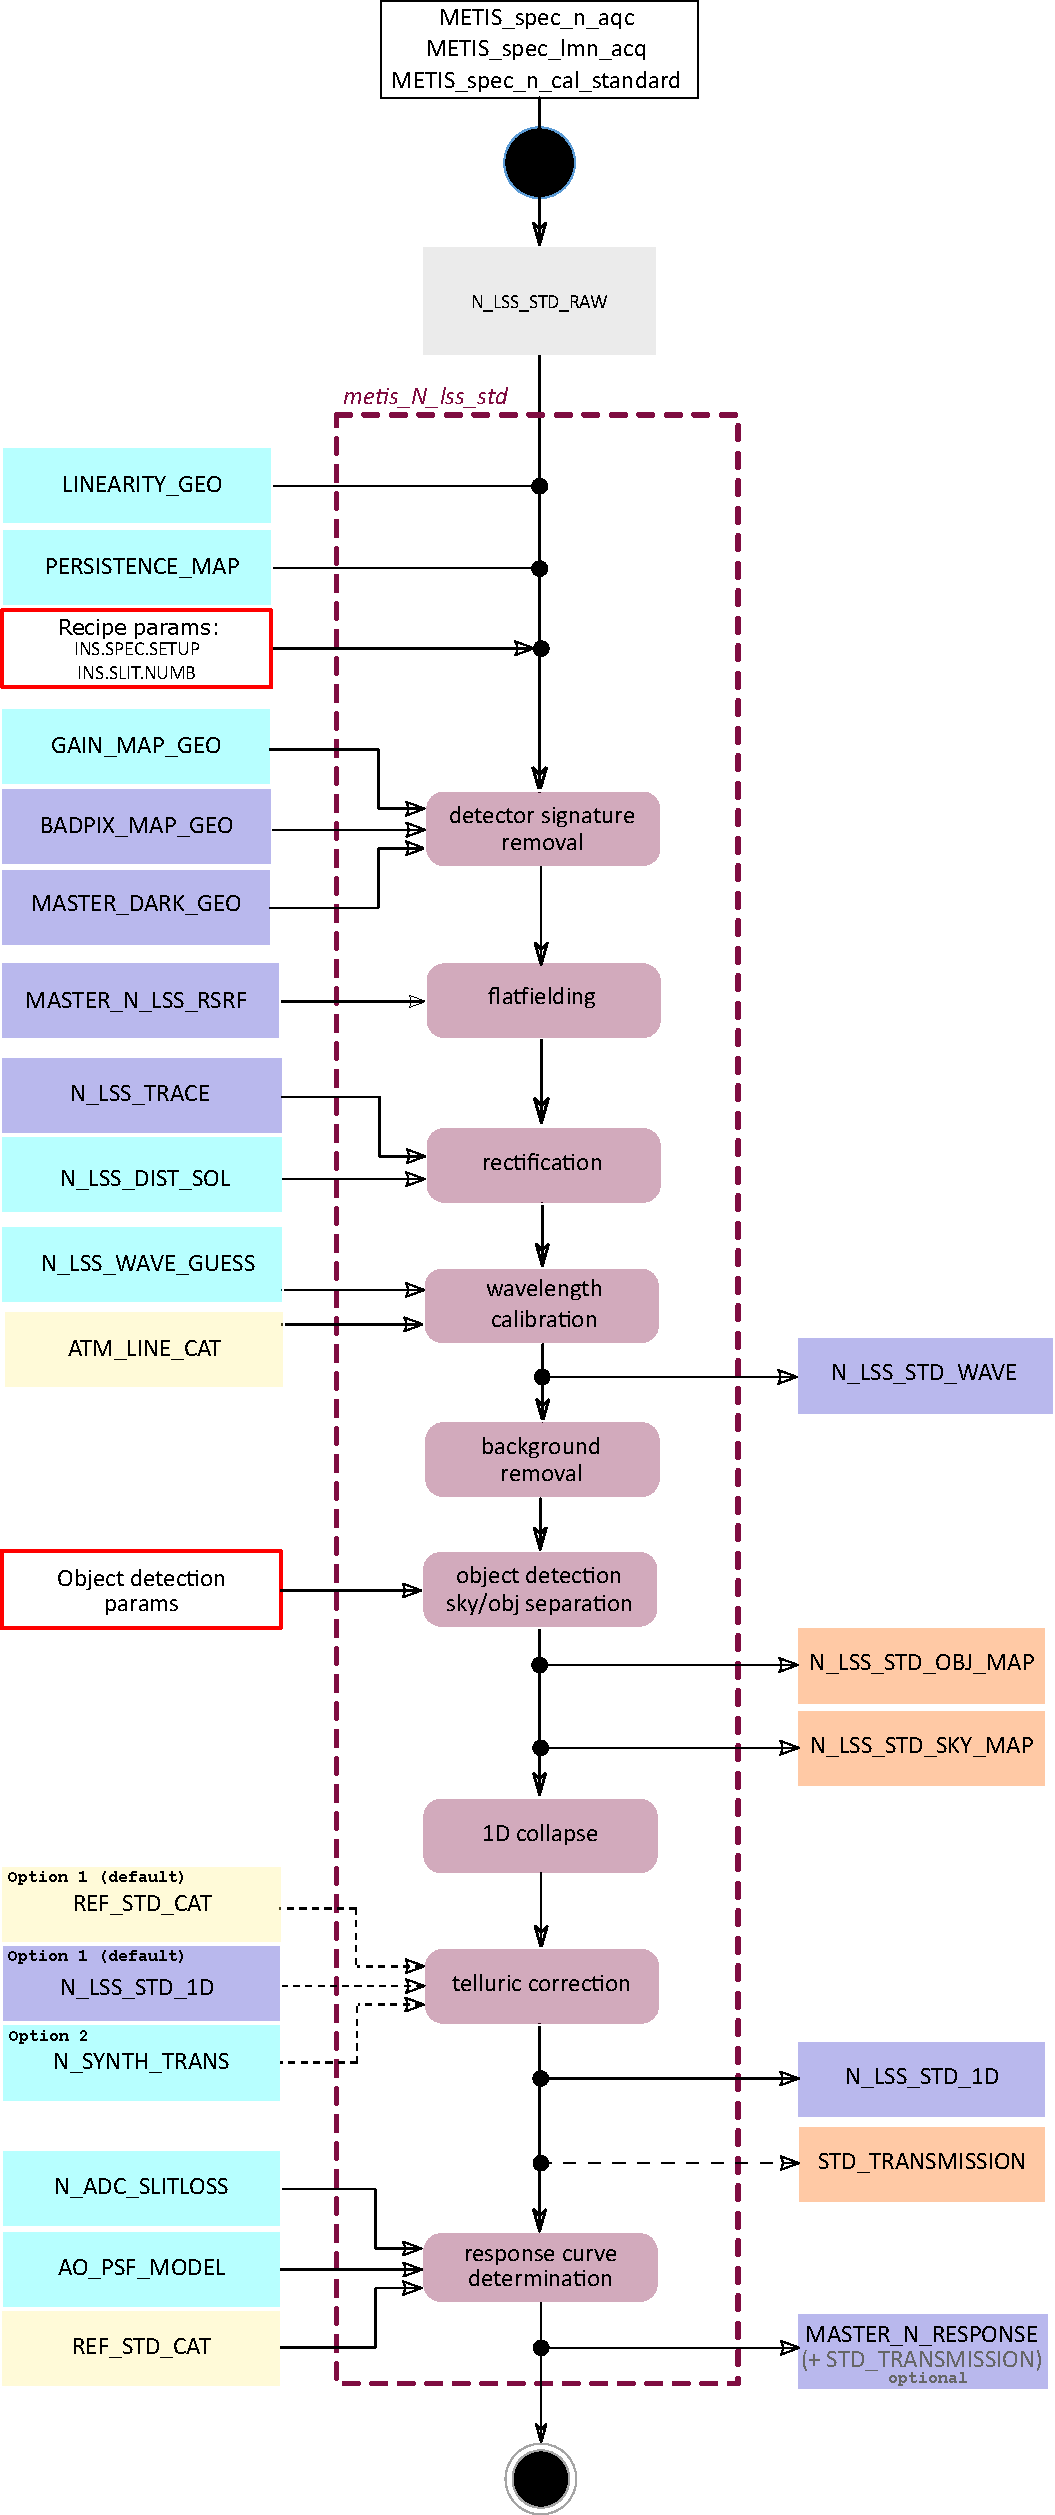
\includegraphics[width=0.4\textheight]{figures/metis_n_lss_std_v0.83.pdf}
  \caption[Recipe: \REC{metis_N_lss_std}]{\REC{metis_N_lss_std} --
    Standard star calibration recipe.}
  \label{Fig:rec_N_lss_flux}
\end{figure}
\clearpage
\begin{recipedef}
Name:		& \hyperref[rec:metis_n_lss_std]{\REC{metis_N_lss_std}} \\
Purpose:	& Flux calibration \\
Type:		& Calibration\\
Requirements: & METIS-6084, METIS-6074 \\
Templates:           & \TPL{METIS_spec_N_cal_standard}\\
Input data: 	& \hyperref[dataitem:n_lss_std_raw]{\RAW{N_LSS_STD_RAW}}\\
                & \hyperref[dataitem:persistence_map]{\EXTCALIB{PERSISTENCE_MAP}}  \\
                & \hyperref[dataitem:linearity_geo]{\STATCALIB{LINEARITY_GEO}}  \\
                & \hyperref[dataitem:gain_map_geo]{\PROD{GAIN_MAP_GEO}}  \\
                & \hyperref[dataitem:badpix_map_geo]{\PROD{BADPIX_MAP_GEO}}   \\
                & \hyperref[dataitem:master_dark_geo]{\PROD{MASTER_DARK_GEO}}  \\
                & \hyperref[dataitem:master_n_lss_rsrf]{\PROD{MASTER_N_LSS_RSRF}} \\
                & \hyperref[dataitem:n_lss_trace]{\PROD{N_LSS_TRACE}}\\
                & \hyperref[dataitem:n_lss_dist_sol]{\STATCALIB{N_LSS_DIST_SOL}} \\
                & \hyperref[dataitem:n_lss_wave_guess]{\STATCALIB{N_LSS_WAVE_GUESS}} \\
                & \hyperref[dataitem:n_synth_trans]{\STATCALIB{N_SYNTH_TRANS}}\\
                & \hyperref[dataitem:ao_psf_model]{\EXTCALIB{AO_PSF_MODEL}} \\
                & \hyperref[dataitem:atm_line_cat]{\EXTCALIB{ATM_LINE_CAT}} \\
                & \hyperref[dataitem:n_adc_slitloss]{\STATCALIB{N_ADC_SLITLOSS}}\\
                & \hyperref[dataitem:ref_std_cat]{\STATCALIB{REF_STD_CAT}} \\                
Parameters: 	& (TBD)\\
Algorithm:      & Application of master calibration files\\
                & Background removal\\
                & Determination and application of the distortion correction\\
                & Determination and application of the wavelength solution\\
                & Identifying/separatiing sky/object pixels\\
                & Removing sky lines: Creation and Subtraction of 2D sky\\
                & Collapsing 2D to 1D spectrum, (see Fig.\,\ref{Fig:rec_N_lss_sci})\\
                & Determination and application of response curve\\
Output data:	& \hyperref[dataitem:n_lss_std_obj_map]{\PROD{N_LSS_STD_OBJ_MAP}}: Pixel map of object pixels (\ac{QC})\\
            	& \hyperref[dataitem:n_lss_std_sky_map]{\PROD{N_LSS_STD_SKY_MAP}}: Pixel map of sky pixels (\ac{QC})\\
              	& \hyperref[dataitem:n_lss_std_1d]{\PROD{N_LSS_STD_1D}}  : coadded, wavelength calibrated, collapsed 1D spectrum\\
                & \hyperref[dataitem:std_transmission]{\PROD{STD_TRANSMISSION}}: Transmission curve derived by menas of the \ac{STD} star (\ac{QC})\\
                & \hyperref[dataitem:master_n_response]{\PROD{MASTER_N_RESPONSE}}: response function (optionally including the transmission)\\
Expected accuracies: & 10\% over an atmospheric band (ESO Req. R-MET-107)\\
            & $<30$\% absolute line flux accuracy (R-MET-107)\\
            & $<5$\% absolute flux calibration (R-MET-82)\\
QC1 parameters: & \hyperref[qc:qc_n_lss_std_backgd_mean]{\QC{QC N LSS STD BACKGD MEAN}}: Mean value of background\\
                & \hyperref[qc:qc_n_lss_std_backgd_median]{\QC{QC N LSS STD BACKGD MEDIAN}}: Median value of background\\
                & \hyperref[qc:qc_n_lss_std_backgd_stdev]{\QC{QC N LSS STD BACKGD STDEV}}: Standard deviation value of background\\
                & \hyperref[qc:qc_n_lss_std_snr]{\QC{QC N LSS STD SNR}}: Signal-to-noise ration of flux standard star spectrum\\
                & \hyperref[qc:qc_n_lss_std_snrnoise]{\QC{QC N LSS STD SNRNOISE}}: Noise level of flux standard star spectrum\\
                & \hyperref[qc:qc_n_lss_std_fwhm]{\QC{QC N LSS STD FWHM}}: FWHM of flux standard spectrum\\
                & \hyperref[qc:qc_n_lss_flux_intordr_level]{\QC{QC N LSS FLUX INTORDR LEVEL}}: Flux level of the interorder background\\
                & \hyperref[qc:qc_n_lss_flux_avglevel]{\QC{QC N LSS FLUX AVGLEVEL}}: Average level of the standard star flux \\
                & \hyperref[qc:qc_n_lss_flux_wavecal_devmean]{\QC{QC N LSS FLUX WAVECAL DEVMEAN}}: Mean deviation from the
                  wavelength reference frame (TBDef)\\
                & \hyperref[qc:qc_n_lss_flux_wavecal_fwhm]{\QC{QC N LSS FLUX WAVECAL FWHM}}: Measured FWHM of lines\\
                & \hyperref[qc:qc_n_lss_flux_wavecal_nident]{\QC{QC N LSS FLUX WAVECAL NIDENT}}: Number of identified lines\\
                & \hyperref[qc:qc_n_lss_flux_wavecal_nmatch]{\QC{QC N LSS FLUX WAVECAL NMATCH}}: Number of lines matched between
                    catalogue and spectrum\\
                & \hyperref[qc:qc_n_lss_flux_wavecal_polydeg]{\QC{QC N LSS FLUX WAVECAL POLYDEG}}: Degree of the polynomial\\
                & \hyperref[qc:qc_n_lss_flux_wavecal_polycoeff<n>]{\QC{QC N LSS FLUX WAVECAL POLYCOEFF<n>}}: $n$-th coefficient of the polynomial\\
                & \hyperref[qc:qc_n_lss_flux_stdsnr]{\QC{QC N LSS FLUX STDSNR}}: Signal-to-noise ration of flux standard star spectrum\\
                & \hyperref[qc:qc_n_lss_flux_snrnoise]{\QC{QC N LSS FLUX SNRNOISE}}: Noise level of flux standard star spectrum\\
                & \hyperref[qc:qc_n_lss_flux_fwhm]{\QC{QC N LSS FLUX FWHM}}: FWHM of flux standard spectrum\\
                & \hyperref[qc:qc_n_lss_flux_psfloss]{\QC{QC N LSS FLUX PSFLOSS}}: Fraction of AO induced slit losses (TBdef)\\
                & more TBD\\
\end{recipedef}

\subsubsection{N-LSS science reduction recipe \REC{metis_N_lss_sci}:}\label{rec:metis_n_lss_sci}
The science calibration recipe comprises the extraction of the object (i.e. separation of object/sky pixels), removing the sky lines, the application of the response curve previously defined, the 2D to 1D collapse and the co-addition. It also applies an absolute flux calibration (optionally with the telluric correction in one step, cf. Section~\ref{ssec:tellcorr}).
\begin{figure}[ht]
  \centering
  \includegraphics[width=0.35\textheight]{figures/metis_N_lss_sci_v0.83.pdf}
  \caption[Recipe: \REC{metis_N_lss_sci}]{\REC{metis_N_lss_sci} --
    Science reduction recipe.}
  \label{Fig:rec_N_lss_sci}
\end{figure}
\clearpage

\begin{recipedef}
Name:		& \hyperref[rec:metis_n_lss_sci]{\REC{metis_N_lss_sci}} \\
Purpose:  & Science data calibration\\
Type:		& Science reduction\\
Requirements: & METIS-6084 \\
Templates:           & \TPL{METIS_spec_N_acq}, \\
                & \TPL{METIS_spec_n_obs_AutoChopNodOnSlit}, \\
% HB 20230627 Template METIS_spec_N_obs_GenericOffset does not exist
%                 & \TPL{METIS_spec_N_obs_GenericOffset} \\
                & \TPL{METIS_spec_n_cal_slit}\\
Input data: 	& \hyperref[dataitem:n_lss_sci_raw]{\RAW{N_LSS_SCI_RAW}}\\
                & \hyperref[dataitem:persistence_map]{\EXTCALIB{PERSISTENCE_MAP}}  \\
                & \hyperref[dataitem:linearity_geo]{\STATCALIB{LINEARITY_GEO}}  \\
                & \hyperref[dataitem:gain_map_geo]{\PROD{GAIN_MAP_GEO}}  \\
                & \hyperref[dataitem:badpix_map_geo]{\PROD{BADPIX_MAP_GEO}}   \\
                & \hyperref[dataitem:master_dark_geo]{\PROD{MASTER_DARK_GEO}}  \\
                & \hyperref[dataitem:master_n_lss_rsrf]{\PROD{MASTER_N_LSS_RSRF}} \\
                & \hyperref[dataitem:n_lss_trace]{\PROD{N_LSS_TRACE}}\\
                & \hyperref[dataitem:n_lss_dist_sol]{\STATCALIB{N_LSS_DIST_SOL}}\\
                & \hyperref[dataitem:n_lss_wave_guess]{\STATCALIB{N_LSS_WAVE_GUESS}}\\
                & \hyperref[dataitem:atm_line_cat]{\EXTCALIB{ATM_LINE_CAT}} \\
                %& \hyperref[dataitem:ao_psf_model]{\EXTCALIB{AO_PSF_MODEL}} \\
                & \hyperref[dataitem:n_adc_slitloss]{\STATCALIB{N_ADC_SLITLOSS}}\\
                & \hyperref[dataitem:master_n_response]{\PROD{MASTER_N_RESPONSE}} \\
Parameters: 	& (TBD)\\
Algorithm:      & Application of the detector master calib files\\
                & wavelength calibration \\
                & Identifying/separatiing sky/object pixels\\
                & Removing sky lines: Creation and Subtraction of 2D sky\\
                & Coaddition of individual object spectra of one OB\\
                & Collapsing 2D to 1D spectrum, (see Fig.\,\ref{Fig:rec_N_lss_sci})\\
                & Application of the response function (flux calibration) \\
Output data:	& \hyperref[dataitem:n_lss_sci_obj_map]{\PROD{N_LSS_SCI_OBJ_MAP}}: Pixel map of object pixels (\ac{QC})\\
            	& \hyperref[dataitem:n_lss_sci_sky_map]{\PROD{N_LSS_SCI_SKY_MAP}}: Pixel map of sky pixels (\ac{QC})\\
            	& \hyperref[dataitem:n_lss_sci_2d]{\PROD{N_LSS_SCI_2D}}: coadded, wavelength calibrated 2D spectrum\\
                & (\FITS{PRO_CATG}: \FITS{N_LSS_2d_coadd_wavecal}) \\
                & \hyperref[dataitem:n_lss_sci_1d]{\PROD{N_LSS_SCI_1D}}: coadded, wavelength calibrated 1D spectrum\\
                & (\FITS{PRO_CATG}: \FITS{N_LSS_1d_coadd_wavecal}) \\
                & \hyperref[dataitem:n_lss_sci_flux_2d]{\PROD{N_LSS_SCI_FLUX_2D}}: coadded, wavelength calibrated 2D spectrum\\
                & (\FITS{PRO_CATG}: \FITS{N_LSS_2d_coadd_wavecal}) \\
              	& \hyperref[dataitem:n_lss_sci_flux_1d]{\PROD{N_LSS_SCI_FLUX_1D}}: coadded, wavelength 1D spectrum\\
                & (\FITS{PRO_CATG}: \FITS{N_LSS_1d_coadd_wavecal}) \\
Expected accuracies: & (TBD)\\
QC1 parameters: & \hyperref[qc:qc_n_lss_sci_snr]{\QC{QC N LSS SCI SNR}}: Signal-to-noise ration of science spectrum\\
                & \hyperref[qc:qc_n_lss_sci_snrnoise]{\QC{QC N LSS SCI SNRNOISE}}: Noise level of science spectrum\\
                & \hyperref[qc:qc_n_lss_sci_flux_snr]{\QC{QC N LSS SCI FLUX SNR}}: Signal-to-noise ration of flux calibrated  science spectrum\\
                & \hyperref[qc:qc_n_lss_sci_flux_snrnoise]{\QC{QC N LSS SCI FLUX SNRNOISE}}: Noise level of flux calibrated science spectrum\\
                & \hyperref[qc:qc_n_lss_sci_intordr_level]{\QC{QC N LSS SCI INTORDR LEVEL}}: Flux level of the interorder background\\
                & \hyperref[qc:qc_n_lss_sci_wavecal_devmean]{\QC{QC N LSS SCI WAVECAL DEVMEAN}}: Mean deviation from the wavelength reference frame (TBDef)\\
                & \hyperref[qc:qc_n_lss_sci_wavecal_fwhm]{\QC{QC N LSS SCI WAVECAL FWHM}}: Measured FWHM of lines\\
                & \hyperref[qc:qc_n_lss_sci_wavecal_nident]{\QC{QC N LSS SCI WAVECAL NIDENT}}: Number of identified lines\\
                & \hyperref[qc:qc_n_lss_sci_wavecal_nmatch]{\QC{QC N LSS SCI WAVECAL NMATCH}}: Number of lines matched between catalogue and spectrum\\
                & \hyperref[qc:qc_n_lss_sci_wavecal_polydeg]{\QC{QC N LSS SCI WAVECAL POLYDEG}}: Degree of the wavelength polynomial\\
                & \hyperref[qc:qc_n_lss_sci_wavecal_polycoeff<n>]{\QC{QC N LSS SCI WAVECAL POLYCOEFF<n>}}: $n$-th coefficient of the polynomial\\
                & more TBD\\
\end{recipedef}

\subsubsection{N-LSS telluric correction recipe \REC{metis_N_lss_mf_model}:}\label{rec:metis_n_lss_mf_model}
The telluric correction will be done with the package \texttt{molecfit}\footnote{\url{https://www.eso.org/sci/software/pipelines/molecfit/molecfit-pipe-recipes.html}}. It is realised in three individual recipes, \hyperref[rec:metis_n_lss_mf_model]{\REC{metis_N_lss_mf_model}}, which calculates the best-fit model, \hyperref[rec:metis_n_lss_mf_calctrans]{\REC{metis_N_lss_mf_calctrans}}, which creates a synthetic transmission curve, and \hyperref[rec:metis_n_lss_mf_correct]{\REC{metis_N_lss_mf_correct}}, which performs the actual telluric correction by means of the synthetic transmission.

\begin{figure}[ht]
  \centering
  \includegraphics[width=0.5\textheight]{figures/metis_N_lss_mf_model_v0.83.pdf}
  \caption[Recipe: \REC{metis_N_lss_mf_model}]{\REC{metis_N_lss_mf_model} --
    Recipe to achieve the best-fit for the calculation of the synthetic transmission curve for the telluric correction.}
  \label{Fig:rec_N_lss_mf_model}
\end{figure}
\clearpage

\begin{recipedef}
Name:		& \hyperref[rec:metis_n_lss_mf_model]{\REC{metis_N_lss_mf_model}}\\
Purpose:	& Achieve the best fit for modelling the transmission curve to be applied as telluric correction \\
Type:		& Post-calibration\\
Requirements: & METIS-4051, METIS-6091 \\
Templates:           & None\\
Input data: 	& \hyperref[dataitem:n_lss_sci_flux_1d]{\PROD{N_LSS_SCI_FLUX_1D}}\\
                & \hyperref[dataitem:lsf_kernel]{\STATCALIB{LSF_KERNEL}} \\
                & \hyperref[dataitem:atm_profile]{\EXTCALIB{ATM_PROFILE}} \\
                & \hyperref[dataitem:atm_line_cat]{\EXTCALIB{ATM_LINE_CAT}} \\
Parameters: 	& \texttt{molecfit} parameters (c.f. \cite{molecfit})\\
Algorithm:      & Fit of telluric features visible in the science input spectrum\\
                & Determination of best-fit parameter set\\
Output data:	& \hyperref[dataitem:mf_best_fit_tab]{\PROD{MF_BEST_FIT_TAB}}\\
Expected accuracies: & (TBD)\\
QC1 parameters: & cf. \cite{molecfit}\\
\end{recipedef}

\subsubsection{N-LSS telluric correction recipe \REC{metis_N_lss_mf_calctrans}:}\label{rec:metis_n_lss_mf_calctrans}
\begin{figure}[ht]
  \centering
  \includegraphics[width=0.5\textheight]{figures/metis_N_lss_mf_calctrans_v0.83.pdf}
  \caption[Recipe: \REC{metis_N_lss_mf_calctrans}]{\REC{metis_N_lss_mf_calctrans} --
    Recipe to calculate the synthetic transmission to be applied as telluric correction.}
  \label{Fig:rec_N_lss_mf_calctrans}
\end{figure}
\clearpage

\begin{recipedef}
Name:		& \hyperref[rec:metis_n_lss_mf_calctrans]{\REC{metis_N_lss_mf_calctrans}}\\
Purpose:	& Calculation of the synthetic transmission \\
Type:		& Post-calibration\\
Requirements: & METIS-4051, METIS-6091 \\
Templates:           & None\\
Input data: 	& \hyperref[dataitem:mf_best_fit_tab]{\PROD{MF_BEST_FIT_TAB}}\\
                & \hyperref[dataitem:lsf_kernel]{\STATCALIB{LSF_KERNEL}} \\
                & \hyperref[dataitem:atm_profile]{\EXTCALIB{ATM_PROFILE}} \\
                & \hyperref[dataitem:atm_line_cat]{\EXTCALIB{ATM_LINE_CAT}} \\
Parameters: 	& \texttt{molecfit} parameters (c.f.  \cite{molecfit})\\
Algorithm:      & Calculate the entire transmission curve by means of the best-fit parameters\\
Output data:	& \hyperref[dataitem:n_lss_synth_trans]{\PROD{N_LSS_SYNTH_TRANS}}\\
\\
Expected accuracies: & (TBD)\\
QC1 parameters: & cf. \cite{molecfit}\\
\end{recipedef}

\subsubsection{N-LSS telluric correction recipe \REC{metis_N_lss_mf_correct}:}\label{rec:metis_n_lss_mf_correct}
\begin{figure}[ht]
  \centering
  \includegraphics[width=0.5\textheight]{figures/metis_N_lss_mf_correct_v0.83.pdf}
  \caption[Recipe: \REC{metis_N_lss_mf_correct}]{\REC{metis_N_lss_mf_correct} --
    Recipe to apply the telluric correction.}
  \label{Fig:rec_N_lss_mf_correct}
\end{figure}
\clearpage

\begin{recipedef}
Name:		& \hyperref[rec:metis_n_lss_mf_correct]{\REC{metis_N_lss_mf_correct}}\\
Purpose:	& Apply the synthetic transmission to the science spectra \\
Type:		& Post-calibration\\
Requirements: & METIS-4051, METIS-6091 \\
Templates:           & None\\
Input data: 	& \hyperref[dataitem:n_lss_sci_flux_1d]{\PROD{N_LSS_SCI_FLUX_1D}}\\
                & \hyperref[dataitem:n_lss_synth_trans]{\PROD{N_LSS_SYNTH_TRANS}}\\
Parameters: 	& None\\
Algorithm:      & Apply telluric correction, i.e. divide the input science spectrum\\
                & by the synthetic transmission\\
Output data:	& \hyperref[dataitem:n_lss_sci_flux_tellcorr_1d]{\PROD{N_LSS_SCI_FLUX_TELLCORR_1D}}\\
Expected accuracies: & (TBD)\\
QC1 parameters: & cf. \cite{molecfit}\\
\end{recipedef}







